\documentclass[border=10pt]{standalone}
\usepackage{tikz}

\begin{document}

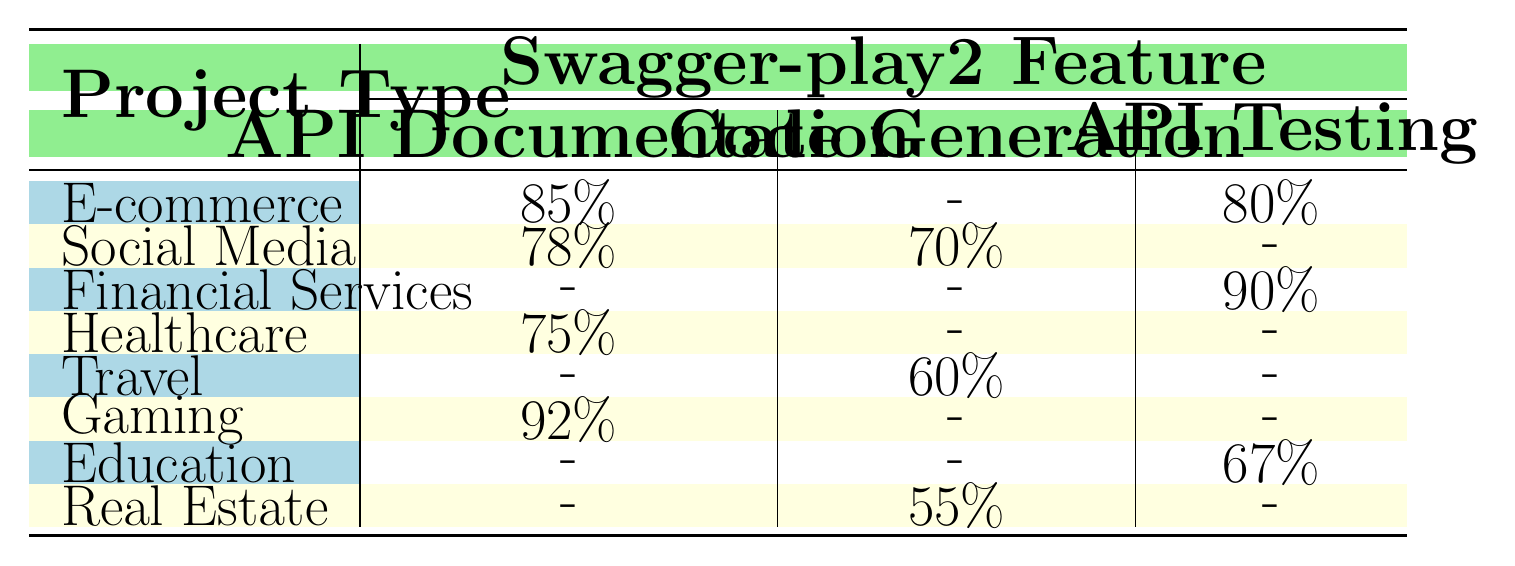
\begin{tikzpicture}[x=1cm,y=1cm]
    \definecolor{headergreen}{RGB}{144,238,144}
    \definecolor{firstcolblue}{RGB}{173,216,230}
    \definecolor{rowyellow}{RGB}{255,255,224}

    % Column boundaries
    \coordinate (O) at (0,0);
    \def\xA{0}
    \def\xB{4.2}
    \def\xC{9.5}
    \def\xD{14.05}
    \def\xE{17.5}

    % Row boundaries
    \def\toprule{0}
    \def\hOneTop{-0.18}
    \def\hOneBottom{-0.78}
    \def\betweenHeaders{-0.88}
    \def\hTwoTop{-1.02}
    \def\hTwoBottom{-1.62}
    \def\headBottom{-1.78}
    \def\bodyTop{-1.92}
    \def\rowH{0.55}
    \def\bodyBottom{-6.32}
    \def\bottomrule{-6.42}

    % Header fills: Project Type is a two-row header; feature title spans three columns
    \fill[headergreen] (\xA,\hOneTop) rectangle (\xE,\hOneBottom);
    \fill[headergreen] (\xA,\hTwoTop) rectangle (\xE,\hTwoBottom);

    % Body striping and first-column highlighting on non-striped rows
    \foreach \i in {0,...,7} {
        \pgfmathsetmacro{\yt}{\bodyTop-\i*\rowH}
        \pgfmathsetmacro{\yb}{\bodyTop-(\i+1)*\rowH}
        \ifodd\i
            \fill[rowyellow] (\xA,\yt) rectangle (\xE,\yb);
        \else
            \fill[firstcolblue] (\xA,\yt) rectangle (\xB,\yb);
        \fi
    }

    % Booktabs-style sparse rules
    \draw[line width=1.2pt] (\xA,\toprule) -- (\xE,\toprule);
    \draw[line width=0.45pt] (\xB,\betweenHeaders) -- (\xE,\betweenHeaders);
    \draw[line width=0.9pt] (\xA,\headBottom) -- (\xE,\headBottom);
    \draw[line width=1.2pt] (\xA,\bottomrule) -- (\xE,\bottomrule);

    % Sparse vertical column rules, with grouped first header row preserved
    \draw[line width=0.55pt] (\xB,\hOneTop) -- (\xB,\bodyBottom);
    \draw[line width=0.55pt] (\xC,\hTwoTop) -- (\xC,\bodyBottom);
    \draw[line width=0.55pt] (\xD,\hTwoTop) -- (\xD,\bodyBottom);

    % Header text
    \node[anchor=west, font=\bfseries\fontsize{24}{26}\selectfont] at (0.28,-0.90) {Project Type};
    \node[font=\bfseries\fontsize{24}{26}\selectfont] at ({(\xB+\xE)/2},-0.48) {Swagger-play2 Feature};
    \node[font=\bfseries\fontsize{24}{26}\selectfont] at ({(\xB+\xC)/2},-1.32) {API Documentation};
    \node[font=\bfseries\fontsize{24}{26}\selectfont] at ({(\xC+\xD)/2},-1.32) {Code Generation};
    \node[font=\bfseries\fontsize{24}{26}\selectfont] at ({(\xD+\xE)/2},-1.32) {API Testing};

    % Body text
    \node[anchor=west, font=\fontsize{22}{24}\selectfont] at (0.28,-2.195) {E-commerce};
    \node[font=\fontsize{22}{24}\selectfont] at ({(\xB+\xC)/2},-2.195) {85\%};
    \node[font=\fontsize{22}{24}\selectfont] at ({(\xC+\xD)/2},-2.195) {-};
    \node[font=\fontsize{22}{24}\selectfont] at ({(\xD+\xE)/2},-2.195) {80\%};

    \node[anchor=west, font=\fontsize{22}{24}\selectfont] at (0.28,-2.745) {Social Media};
    \node[font=\fontsize{22}{24}\selectfont] at ({(\xB+\xC)/2},-2.745) {78\%};
    \node[font=\fontsize{22}{24}\selectfont] at ({(\xC+\xD)/2},-2.745) {70\%};
    \node[font=\fontsize{22}{24}\selectfont] at ({(\xD+\xE)/2},-2.745) {-};

    \node[anchor=west, font=\fontsize{22}{24}\selectfont] at (0.28,-3.295) {Financial Services};
    \node[font=\fontsize{22}{24}\selectfont] at ({(\xB+\xC)/2},-3.295) {-};
    \node[font=\fontsize{22}{24}\selectfont] at ({(\xC+\xD)/2},-3.295) {-};
    \node[font=\fontsize{22}{24}\selectfont] at ({(\xD+\xE)/2},-3.295) {90\%};

    \node[anchor=west, font=\fontsize{22}{24}\selectfont] at (0.28,-3.845) {Healthcare};
    \node[font=\fontsize{22}{24}\selectfont] at ({(\xB+\xC)/2},-3.845) {75\%};
    \node[font=\fontsize{22}{24}\selectfont] at ({(\xC+\xD)/2},-3.845) {-};
    \node[font=\fontsize{22}{24}\selectfont] at ({(\xD+\xE)/2},-3.845) {-};

    \node[anchor=west, font=\fontsize{22}{24}\selectfont] at (0.28,-4.395) {Travel};
    \node[font=\fontsize{22}{24}\selectfont] at ({(\xB+\xC)/2},-4.395) {-};
    \node[font=\fontsize{22}{24}\selectfont] at ({(\xC+\xD)/2},-4.395) {60\%};
    \node[font=\fontsize{22}{24}\selectfont] at ({(\xD+\xE)/2},-4.395) {-};

    \node[anchor=west, font=\fontsize{22}{24}\selectfont] at (0.28,-4.945) {Gaming};
    \node[font=\fontsize{22}{24}\selectfont] at ({(\xB+\xC)/2},-4.945) {92\%};
    \node[font=\fontsize{22}{24}\selectfont] at ({(\xC+\xD)/2},-4.945) {-};
    \node[font=\fontsize{22}{24}\selectfont] at ({(\xD+\xE)/2},-4.945) {-};

    \node[anchor=west, font=\fontsize{22}{24}\selectfont] at (0.28,-5.495) {Education};
    \node[font=\fontsize{22}{24}\selectfont] at ({(\xB+\xC)/2},-5.495) {-};
    \node[font=\fontsize{22}{24}\selectfont] at ({(\xC+\xD)/2},-5.495) {-};
    \node[font=\fontsize{22}{24}\selectfont] at ({(\xD+\xE)/2},-5.495) {67\%};

    \node[anchor=west, font=\fontsize{22}{24}\selectfont] at (0.28,-6.045) {Real Estate};
    \node[font=\fontsize{22}{24}\selectfont] at ({(\xB+\xC)/2},-6.045) {-};
    \node[font=\fontsize{22}{24}\selectfont] at ({(\xC+\xD)/2},-6.045) {55\%};
    \node[font=\fontsize{22}{24}\selectfont] at ({(\xD+\xE)/2},-6.045) {-};
\end{tikzpicture}

\end{document}
